\section{Results}\label{sec:results}

\subsection{Degradation by circuit and compound}\label{sec:rates}

Degradation varies about twice as much between circuits, and between races, as between compounds.
Pooling 2022 to 2026 (\PooledNEvents{} races at \PooledNCircuits{} circuits, \PooledNRepeat{} of them raced more than once; \PooledNLaps{} laps in \PooledNRuns{} runs), the tyre-age slope has a persistent circuit component with standard deviation \PersistSD\spl{} (95\% profile interval [\PersistSDLo, \PersistSDHi]; parametric bootstrap [\PersistSDBootLo, \PersistSDBootHi]), a difference of \PersistSDsPerTwenty\,s [\PersistSDsPerTwentyLo, \PersistSDsPerTwentyHi] in lap time at a tyre age of 20 laps.
Race-to-race variation at the same circuit is about as large: \EventSD\spl{} [\EventSDLo, \EventSDHi], or \EventSDsPerTwenty\,s at 20 laps.
The persistent share of the between-race slope variance is \PersistShare{} (bootstrap interval [\PersistShareBootLo, \PersistShareBootHi]), so about half of the variation between races is shared by the races at a circuit (Figure~\ref{fig:decomp}A).
Slopes vary still more between runs within a race (standard deviation \RunSlopeSD\spl), which is why the intervals must count runs.
The likelihood-ratio statistic for no persistent circuit component is \PooledLRCircuit{}, with a bootstrap $p$-value of \PooledPCircuit{}, the smallest that \PooledNBootCircuit{} replicates can give; for no race-specific component it is \PooledLREvent.
Dropping 2025, whose compound numbers were re-specified, or keeping only verified nominations leaves the persistent standard deviation at \SensNoTwentyFiveCircuitSD{} and \SensVerifiedCircuitSD\spl.

The compounds differ too, in the expected order but by less.
The pooled rates are \PooledRateCOne{} and \PooledRateCTwo\spl{} for C1 and C2 and rise to \PooledRateCThree, \PooledRateCFour{} and \PooledRateCFive\spl{} for C3 to C5 (Figure~\ref{fig:decomp}B).
Each step from C2 to C5 is detected: C3 minus C2 is \PoolConThreeTwo\spl{} [\PoolConThreeTwoLo, \PoolConThreeTwoHi], C4 minus C3 is \PoolConFourThree{} [\PoolConFourThreeLo, \PoolConFourThreeHi] and C5 minus C4 is \PoolConFiveFour{} [\PoolConFiveFourLo, \PoolConFiveFourHi], whereas C1 and C2 cannot be told apart (\PoolConTwoOne{} [\PoolConTwoOneLo, \PoolConTwoOneHi]).
The standard deviation of the five rates is \PooledCompoundSD\spl{} (bootstrap [\PooledCompoundSDBootLo, \PooledCompoundSDBootHi]), or \PooledCompoundSDCorr\spl{} once sampling noise is removed, so the persistent circuit and race-specific components are each about twice the compound spread.
The persistent circuit standard deviation exceeds the compound one by \CircMinusCompound\spl{} (bootstrap median; [\CircMinusCompoundLo, \CircMinusCompoundHi]), with bootstrap probability \CircGreaterCompoundP{} that the difference is positive.

\begin{figure}[t]
\centering
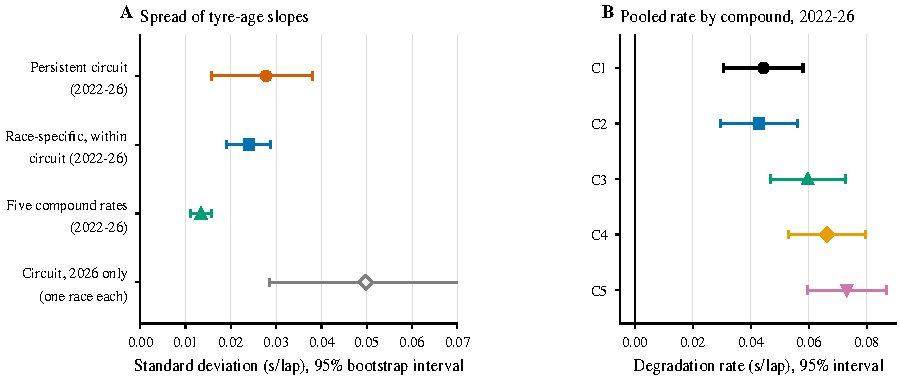
\includegraphics[width=\linewidth]{figures/fig_circuit_decomposition.pdf}
\caption{(A) Standard deviation of the tyre-age slope: persistent circuit and race-specific (event within circuit) components from the pooled 2022--26 model, the standard deviation of the five pooled compound rates, and the circuit standard deviation of the 2026 model alone, in which each circuit is raced once and the two components cannot be separated. Bars are 95\% parametric-bootstrap percentile intervals. (B) Pooled race degradation rate per compound over 2022--26 with 95\% Wald intervals; the marker shapes for compounds are those of Figure~\ref{fig:circuit}.}
\label{fig:decomp}
\end{figure}

A single season gives a less clear picture.
The 2026 season alone has a circuit standard deviation of \CircuitSD\spl{} (profile interval [\CircuitSDLo, \CircuitSDHi]; bootstrap [\CircuitSDBootLo, \CircuitSDBootHi], as in Figure~\ref{fig:decomp}A), larger than either pooled component because each 2026 circuit was raced once, so its slope mixes persistent and race-specific variation.
Its compound rates, from Eq.~\eqref{eq:race} on \NLapsRaceFit{} laps in \NRunsRaceFit{} runs by \NDriversRaceFit{} drivers at \NCircuitsRaceFit{} circuits (Figure~\ref{fig:circuit}A, Appendix Table~\ref{tab:rates}), run from \RateCTwo\spl{} (C2) to \RateCFour\spl{} (C4), with a standard deviation of \CompoundRateSD\spl{} that is no larger than sampling noise alone would produce.
C3 degrades faster than C2, by \SixConThreeTwo\spl{} [\SixConThreeTwoLo, \SixConThreeTwoHi], and C4 faster than C3, by \SixConFourThree{} [\SixConFourThreeLo, \SixConFourThreeHi], but C5 degrades more slowly than C4 (\ContrastCFiveCFour\spl{} [\ContrastCFiveCFourLo, \ContrastCFiveCFourHi]), and C1 and C2 cannot be told apart.
The order also varies between seasons.
Within the same race, softer compounds degrade faster in 2022 (\TrendSeasonTwentyTwo\spl{} per step softer [\TrendSeasonTwentyTwoLo, \TrendSeasonTwentyTwoHi]), 2023 and 2025, but not detectably in 2024 or 2026 (\WithinEventTrend\spl{} [\WithinEventTrendLo, \WithinEventTrendHi]; Appendix Table~\ref{tab:seasons}).
We do not know why the soft end of 2026 differs; candidates are compound-by-phase pace offsets, selection into who stays out, and the 2026 regulations.

\begin{figure}[t]
\centering
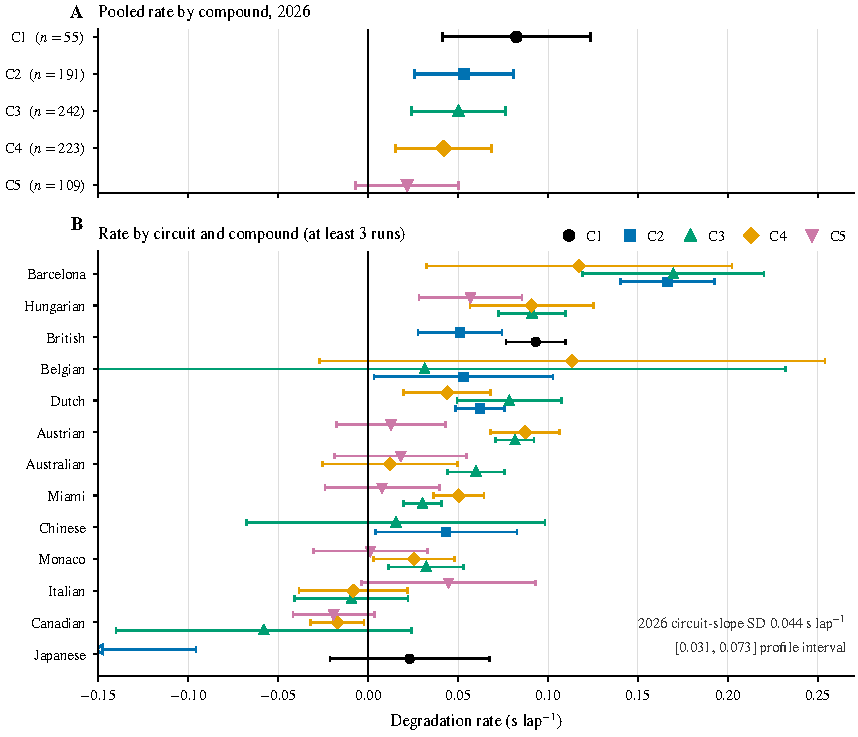
\includegraphics[width=\linewidth]{figures/fig_circuit_rates.pdf}
\caption{(A) Pooled race degradation rate per compound in 2026 with 95\% intervals; $n$ is the number of runs. (B) Separate fits for each circuit and compound with at least three runs, with 95\% run-clustered intervals, circuits ordered by mean rate. Markers: C1 circle, C2 square, C3 upward triangle, C4 diamond, C5 downward triangle. The axis is truncated: intervals are clipped at its edges, and an estimate beyond an edge is shown as an open arrowhead there. The annotation gives the 2026 circuit-slope standard deviation with its 95\% profile-likelihood interval; each circuit is raced once, so it mixes persistent and race-specific variation.}
\label{fig:circuit}
\end{figure}

Without adjustment the estimates are not just noisier but wrong in sign.
A naive regression of lap time on tyre age, with no controls, gives negative degradation for C1, C3 and C5 (\NaiveCOne, \NaiveCThree{} and \NaiveCFive\spl).
A regression that corrects for fuel within runs comes much closer, differing from Eq.~\eqref{eq:race} by \AblGapCThree\spl{} at C3 to \AblGapCOne\spl{} at C1, so most of the gain over the naive fit comes from controlling fuel and run (Appendix~\ref{app:ablation}).
In the recovery study, where the truth is known, the fuel-corrected estimator understates degradation by \RecFuelExoBiasAbs\spl{} on average even with the correct fuel constant, whereas Eq.~\eqref{eq:race} is within 0.002\spl{} of the truth on average when stops are random or depend on car pace; when stops are triggered by wear, both understate it, Eq.~\eqref{eq:race} by \RecExactWearBiasAbs\spl{} (Appendix~\ref{app:recovery}).

\subsection{Calibration of the intervals}\label{sec:calib}

The intervals are close to calibrated, though somewhat narrow for a new circuit, and only because they count runs and circuits rather than laps.
Treating laps as independent and omitting circuit slopes gives intervals only \WidthNoCircuitCThree{} (C3) to \WidthNoCircuitCOne{} (C1) times as wide as the lap-level circuit model; adding run intercepts and slopes widens them further, to \WidthShippedCOne{} (C1) to \WidthShippedCThree{} (C3) times, and cuts the residual lag-1 autocorrelation within runs from \LagOneCircuitModel{} to \LagOneShipped{} (Appendix~\ref{app:inference}).
Leaving each circuit out in turn, the nominal 80\% predictive interval covers the circuit's own fitted rate in \CovEightyLOCO{} of \CovEightyN{} circuit--compound groups (\CovEightyK{} of \CovEightyN{}; Wilson 95\% interval [\CovEightyWilsonLo, \CovEightyWilsonHi]; \citealp{brown2001interval}), and the nominal 95\% interval in \CovNinetyFiveLOCO; without the circuit variance, 80\% coverage falls to \CovEightyNoCircuit.
In simulations from the fitted model, 80\% coverage is \CovEightySBC, which checks the estimator against its own model but cannot reveal misspecification.
In the recovery study, whose data-generating process differs from the model, the nominal 95\% intervals for the compound rates cover the truth in \RecExactExoCov{} and \RecExactPaceCov{} of replicates when stops are random or depend on pace (lowest compound \RecExactPaceWorstCov), and in \RecExactWearCov{} when stops are triggered by wear.

\subsection{What can public timing data separate?}\label{sec:power}

How finely the data separate compounds depends on how many races two compounds share.
From the fitted models' own standard errors, the pooled 2022--26 data would detect, with 80\% power, a gap between neighbouring compounds of \PoolMDEFourThree\spl{} (C3 against C4) to \PoolMDETwoOne\spl{} (C1 against C2), and the 2026 season alone one of \SixMDEFourThree{} to \SixMDETwoOne\spl.
The C1 against C2 pair is the weakest link in both because C1 is nominated at few races; in 2026 the two compounds ran in only six races, and a $t$ reference with that many independent races raises the limit to \SixMDETTwoOne\spl.

To see how the allocation sets these limits, we plant a compound gap in races simulated from the fitted model, refit, and apply the Wald test of Section~\ref{sec:rates}.
Under Pirelli's actual 2026 nominations the C1 against C2 pair, with our \NRunsCOneCTwo{} runs, has a minimum detectable effect of \MDERealCOneCTwo\spl{} (other pairs \MDERealCThreeCFour{} to \MDERealCFourCFive\spl; Figure~\ref{fig:power}B), and simulations that refit the variances agree (\MDESimRealCOneCTwo\spl, Monte Carlo 95\% interval [\MDESimRealCOneCTwoLo, \MDESimRealCOneCTwoHi]); the simulated runs are idealised, with 20 laps each, so these limits are lower than the fitted ones.
Raising the run-slope standard deviation by half lifts the limit to \MDERealCOneCTwoStress\spl, while the ends of the circuit interval change it by less than 0.001\spl.
A gap of \PowerEffectSize\spl, about the hard-to-medium gap reported by \citet[Table~5]{cappelloHoegh2026}, needs \PXRunsRealSix{} runs of the two compounds under the actual allocation and \PXRunsBalSix{} if both ran at every circuit; a gap of 0.02\spl{} needs \PXRunsRealTwenty{} and \PXRunsBalTwenty{} (Figure~\ref{fig:power}A).
If the compounds ran at disjoint circuits, the circuit variance would enter the contrast and no number of runs would suffice: the minimum detectable effect at \NStintsBalanced{} runs is \MDESplit\spl, and power for a gap of 0.03\spl{} cannot exceed \PXSplitCeilThirty.
At zero effect the Wald test rejects in \PXSizeBal{} (balanced) and \PXSizeReal{} (realistic) of \PXSizeReps{} replicates, close to the nominal 0.05; a more conservative $t$ reference (12 degrees of freedom) puts the C1 against C2 limit at \MDESimRealCOneCTwoT\spl.
Simulated run requirements match the analytic ones at every effect size (Figure~\ref{fig:power}A), and the \PowerStintsCappello{} runs available to a single-driver, single-race fit fall far below all of them.

\begin{figure}[t]
\centering
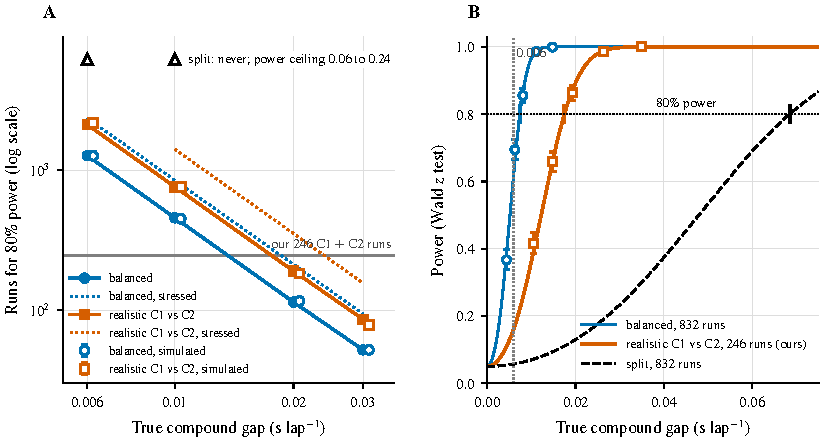
\includegraphics[width=\linewidth]{figures/fig_power.pdf}
\caption{(A) Runs of the two compared compounds needed for 80\% power against the true gap, on log axes. Solid lines are analytic (known variances): the balanced design, with both compounds at every circuit (circles), and the realistic design, Pirelli's actual 2026 nominations for C1 against C2 (squares). Dotted lines use the upper end of the circuit interval and 1.5 times the run-slope standard deviation; points beyond the grid searched are omitted. Open symbols are 80\% crossings in simulations that refit the variances and apply the Wald $z$ test (\PXSimReps{} replicates per point, up to 2{,}000 runs), with Monte Carlo 95\% intervals. The horizontal line marks our \NRunsCOneCTwo{} C1 and C2 runs. In the split design, with the compounds at disjoint circuits, power never reaches 80\% (triangles; ceiling in the label). (B) Power against the true gap at the run counts we hold: analytic curves, simulated points (\MDESimReps{} replicates each) with $\pm1.96$ Monte Carlo standard errors, and ticks at the analytic minimum detectable effect. Balanced and split curves are at \NStintsBalanced{} runs.}
\label{fig:power}
\end{figure}

\subsection{Race versus practice degradation}\label{sec:gap}

On matched used sets, races degrade less than practice, but we cannot attribute the difference to tyre management.

\textit{The gap.}\ On used sets in both settings, the pooled medium and soft race slope is \MatchedRaceSlopeMS\spl{} and the practice slope \MatchedPracticeSlopeMS\spl{} (\NMatchedCellsMS{} groups; Figure~\ref{fig:gap}A).
The gap is \LevelGapMS\spl{} [\LevelGapMSLo, \LevelGapMSHi]; it does not depend on the assumed fuel correction, which cancels in the difference.
The ratio does depend on it: under the assumed correction race degradation is \RaceToPracticeRatio{} of practice degradation (95\% bootstrap interval [\RaceToPracticeRatioLo, \RaceToPracticeRatioHi]), and Appendix~\ref{app:sens} varies the constants.
The point estimates are negative for each compound (\GapHard\spl{} for hard, \GapMedium\spl{} for medium and \GapSoft\spl{} for soft), but only the soft interval excludes zero (Appendix Table~\ref{tab:racepractice}); over all \NMatchedCellsAll{} groups in \NMatchedEventSeasons{} event-seasons the gap is \LevelGapAll\spl{} [\LevelGapAllLo, \LevelGapAllHi].
Every other design agrees in sign, with ratios from \StartAgeRatioMS{} (start-age matching) to \IntersectRatioMS{} (used sets and start age together; Figure~\ref{fig:gap}B).

The placebo shows how large a gap the design can produce by itself.
FP2 against FP1 and FP3 together, on used sets, gives \PlaceboGapMS\spl{} [\PlaceboGapMSLo, \PlaceboGapMSHi] for medium and soft over \NPlaceboCellsMS{} groups, about \PlaceboShareMS{} of the race--practice gap in size.
Subtracting it leaves \PlaceboAdjGapMS\spl{} [\PlaceboAdjGapMSLo, \PlaceboAdjGapMSHi], an interval that includes the placebo's own uncertainty and reaches zero, so differences between sessions such as run plans, fuel and conditions may explain part of the gap.

\begin{figure}[t]
\centering
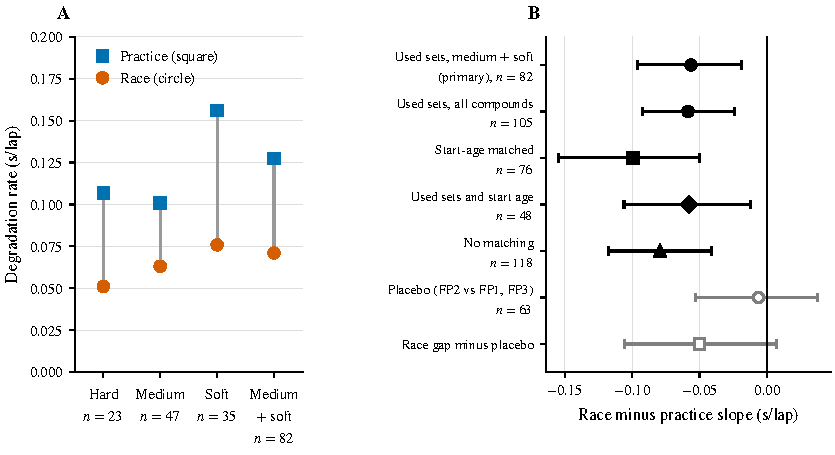
\includegraphics[width=\linewidth]{figures/fig_race_practice.pdf}
\caption{(A) Pooled race (circle) and practice (square) slopes by compound on used sets in both settings; $n$ is the number of groups. (B) Race minus practice slope with 95\% cluster-bootstrap intervals over event-seasons, for medium and soft groups unless stated: the primary design (filled circle), all compounds (filled circle), start-age matching (filled square), used sets and start age together (filled diamond), no matching (filled triangle), and the placebo comparison of FP2 with FP1 and FP3 (open circle) and the race gap minus the placebo gap (open square).}
\label{fig:gap}
\end{figure}

\textit{Is the gap tyre management?}\ The data do not show that it is.
If drivers manage softer tyres more, the gap should grow with softness, and it does not do so reliably, although the tests are underpowered.
In the difference in differences, soft minus hard is \DidTWFESoftHard\spl{} [\DidTWFESoftHardLo, \DidTWFESoftHardHi] over \DidTWFESoftHardNEvents{} events (permutation $p=\DidTWFESoftHardPPerm$, Holm-adjusted $p=\DidTWFESoftHardHolmP$); the other two pairs have intervals that include zero, and soft and medium barely differ, so the pattern is a step between hard and the other compounds rather than a gradient (Appendix Table~\ref{tab:racepractice}).
A uniform damping of every compound by the same factor would itself produce a gradient, because softer tyres have larger practice slopes: a factor of 0.5 implies \UniformDampingImplied\spl{} per step, against \UniformDampingObserved\spl{} observed.
The placebo also produces a gradient, with a soft-minus-medium gap of \PlaceboSoftMedium\spl{} [\PlaceboSoftMediumLo, \PlaceboSoftMediumHi] between practice sessions.

The primary test, the group-level trend of the gap on softness, gives \NursingTrend\spl{} per step [\NursingTrendLo, \NursingTrendHi] with one-sided permutation $p=\NursingPOneSided$ and two-sided $p=\NursingPTwoSided$, so its decision rule is not met.
Its minimum detectable effect at 80\% power is \NursingMDE\spl, more than twice the estimate, so the test cannot rule out an effect of that size.
Of the \MultiverseSpecs{} exploratory specifications, \MultiverseNegative{} give a negative trend and \MultiverseExcludesZero{} have intervals that exclude zero (Appendix~\ref{app:sens}).
Telemetry gives no support either (Appendix~\ref{app:tele}): tyre management predicts more lift-and-coast before braking zones in races than in practice, more so on softer compounds, but the slope of the race-minus-practice change in coasting time on softness is \TelePrimarySlope\,s per step [\TelePrimarySlopeLo, \TelePrimarySlopeHi] over \TelePrimaryNEventsTrend{} events in 2025--2026 (two-sided $p=\TelePrimaryPTwoSided$), and \TeleExtensionSlope\,s per step [\TeleExtensionSlopeLo, \TeleExtensionSlopeHi] over \TeleExtensionNEventsTrend{} events in 2023--2024, nominally in the opposite direction.

\subsection{Can practice predict race degradation?}\label{sec:transfer}

Practice forecasts beat a naive forecast but not a constant one.
Out of season, the scaled forecast has a mean absolute error of \MaeScalar\spl{} (95\% interval [\MaeScalarLo, \MaeScalarHi]) against \MaeNaive\spl{} [\MaeNaiveLo, \MaeNaiveHi] for the naive forecast and \MaeZero\spl{} for predicting zero (Figure~\ref{fig:forecast}).
A constant, the median race rate of other weekends, scores \MaeConstant\spl: the scaled forecast's error exceeds the constant's by \DiffScalarVsConstant\spl{} [\DiffScalarVsConstantLo, \DiffScalarVsConstantHi], and its difference from last season's race rate at the same circuit is \DiffScalarVsHistory\spl{} [\DiffScalarVsHistoryLo, \DiffScalarVsHistoryHi], both indistinguishable from zero.
A compound-specific factor does worse (\MaeCompound\spl), and neither a 50\% shrink towards the constant (\MaeShrink\spl) nor a stack of baselines (\MaeStack\spl) is detectably better (Appendix Table~\ref{tab:forecast}).
In 2026 the tuned error is \MaeTwentySixScalar\spl{} against \MaeTwentySixNaive\spl{} for the naive forecast; selecting the design and weights inside each training fold gives \MaeNested\spl, so tuning flatters the forecast by \NestedOptimism\spl.
Practice therefore removes most of the naive error but carries little information beyond a constant prior, and the choices made in cleaning practice runs hardly matter (Appendix~\ref{app:sens}).

\begin{figure}[t]
\centering
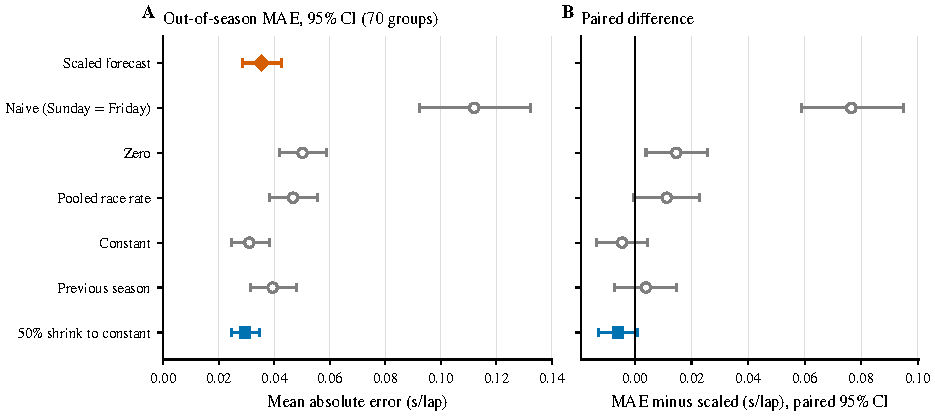
\includegraphics[width=\linewidth]{figures/fig_forecast.pdf}
\caption{Out-of-season (2022--2025) forecasts of race degradation in \HoldoutCells{} event-compound groups. (A) Mean absolute error with 95\% weekend-bootstrap intervals; (B) paired difference of each forecast's error minus the scaled forecast's, with 95\% intervals, so positive values favour the scaled forecast. The scaled forecast is the filled diamond and the 50\% shrink the filled square; all other forecasts are open circles.}
\label{fig:forecast}
\end{figure}

\subsection{Comparison with a published state-space forecaster}\label{sec:bench}

For forecasting a single driver's next lap, the state-space model of \citet{cappelloHoegh2026} is better than our pooled estimator.
Their model conditions on one driver's own history, whereas ours pools every car's laps to estimate a degradation rate; we scored both on their test laps (Appendix~\ref{app:bench}).
Over \BenchNRaces{} races the mean continuous ranked probability score (CRPS, lower is better) is \BenchCRPSSSM{} s for theirs against \BenchCRPSOurs{} s for ours, a paired difference of \BenchDiffSSM{} s [\BenchDiffSSMLo, \BenchDiffSSMHi], and ours wins \BenchWinsVsRepoSSM{} races (sign test $p=\BenchSignPSSM$).
Against their AR(1) benchmark ours wins \JournalWinsAR{} of \JournalRacesScored{} races with a CRPS difference of \JournalDiffAR{} s [\JournalDiffARLo, \JournalDiffARHi], so the two cannot be told apart.
A hierarchical state-space model with several drivers and circuit effects, as the authors suggest (p.~12), could combine both strengths.
